% Standalone: place this file beside the extracted sampling_tau_output folder.
% The figures are the existing PNGs; no analysis or figure generation is needed.
%
% To include in a guide: load graphicx in the guide preamble, then use
%   \def\SamplingTutorialEmbedded{1}
%   \input{path/to/tutorial_sampling_design.tex}
% after the guide's \appendix command (if applicable).
% Figure paths are relative to the document's compilation directory. Override
% the default before \input if needed, for example:
%   \def\SamplingTutorialFigureDir{docs/tutorial/generated/normalized_logistic}
%\ifdefined\SamplingTutorialEmbedded
%  \let\SamplingTutorialEnd\relax
%\else
%  \documentclass[11pt]{article}
%  \usepackage[margin=1in]{geometry}
%  \usepackage{graphicx}
%  \setlength{\parskip}{0.4em}
%  \setlength{\parindent}{0pt}
%  \newcommand{\SamplingTutorialEnd}{\end{document}}
%  \begin{document}
%\fi

%\providecommand{\SamplingTutorialFigureDir}{sampling_tau_output/normalized_logistic}

\section{Worked Example: Sampling Times, Noise, and Model Uncertainty}
\label{sec:sampling-design-tutorial}

\subsection{Purpose and setup}

How well can a fitted curve recover behavior between observations? This example
uses a known synthetic decay to explore how time-point placement, measurement
noise, and replicate count affect that recovery. It complements model comparison:
even when the correct curve form is available, the observations may provide too
little information to determine its shape reliably.

The synthetic fraction remaining follows the normalized logistic model,
\[
  F(t)=\frac{1}{1+\exp\!\left((t-t_{50})/s\right)},
  \qquad t_{50}=50,\quad s=8.
\]
Here, $t_{50}$ is the time at which half remains, and $s$ controls the transition
width. The upper and lower asymptotes are fixed at 1 and 0; $t_{50}$ and $s$ are
fitted using the app's model-fitting machinery. Time is in illustrative units.

Each sampling condition was simulated 100 times with independent Gaussian
measurement errors and fitted with the same logistic model. Standardized errors
were shared across conditions to aid comparison. A separate simulated
study supplies the illustrative observations. Each replicate is an independent
measurement at its assigned time; noise also applies at time zero. The response
scale is fixed, rather than obtained by dividing by a noisy initial observation,
and noisy observations are not clipped to the range 0--1.

\begin{table}[htbp]
  \centering
  \small
  \caption{Sampling conditions. Panel letters refer to
    Figure~\ref{fig:sampling-design-curves}. Noise SD is on the fraction-remaining scale.}
  \label{tab:sampling-design-conditions}
  \renewcommand{\arraystretch}{1.1}
  \begin{tabular}{@{}lp{0.28\linewidth}lcc@{}}
    \hline
    Panels & Condition & Times & Replicates/time & Noise SD \\
    \hline
    A, B & Reference          & 0, 20, 40, 100         & 1 & 0.03 \\
    C    & Misplaced focus    & 0, 10, 20, 100         & 1 & 0.03 \\
    E    & Transition focus   & 0, 40, 60, 100         & 1 & 0.03 \\
    G    & More time points   & 0, 20, 40, 60, 80, 100 & 1 & 0.03 \\
    D    & Higher noise       & 0, 20, 40, 100         & 1 & 0.09 \\
    F    & More replicates, higher noise & 0, 20, 40, 100 & 3 & 0.09 \\
    H    & More times, higher noise & 0, 20, 40, 60, 80, 100 & 1 & 0.09 \\
    \hline
  \end{tabular}
\end{table}

The reference is a deliberately simple, sparse schedule, resembling an in vivo
time course with several early observations and fewer later observations. Its
times are illustrative, rather than a recommended protocol.

\subsection{What the fitted curves show}

\textbf{A convincing individual fit can hide weak support between observations.}
The reference fit in Figure~\ref{fig:sampling-design-curves}A follows the observed
points closely. Across repeated studies, however, the fitted transition varies
substantially (B). Moving the early observations farther from the transition
(``misplaced focus,'' C) leaves even greater freedom in when and how rapidly the
decline occurs. Agreement with the available observations does not establish the
behavior within the long unsampled interval.

\textbf{Moving a time point can be as useful as adding time points.}
Replacing time 20 with time 60 places observations on both sides of the main
transition (E). Recovery improves markedly with the same number of observations.
Adding times 60 and 80 to the reference also improves recovery (G). Both schedules
track the true curve closely, with much less variation between studies. Their
success reflects coverage of the changing part of the curve, rather than simply
a larger sample count.

\textbf{Replicates help with noise, but leave gaps in time coverage.}
Higher measurement noise worsens recovery under the reference schedule (D).
Additional replicates at those same times improve recovery somewhat (F), but
substantial uncertainty about the transition remains. Adding informative times
instead gives more consistent recovery (H), despite using fewer total
observations than the triplicate schedule. Better coverage also partly offsets
the increased noise when compared with the original reference (B). These results
show the importance of placement in this example; they do not imply that
replication or measurement precision is generally unimportant.

\begin{figure}[p]
  \centering
  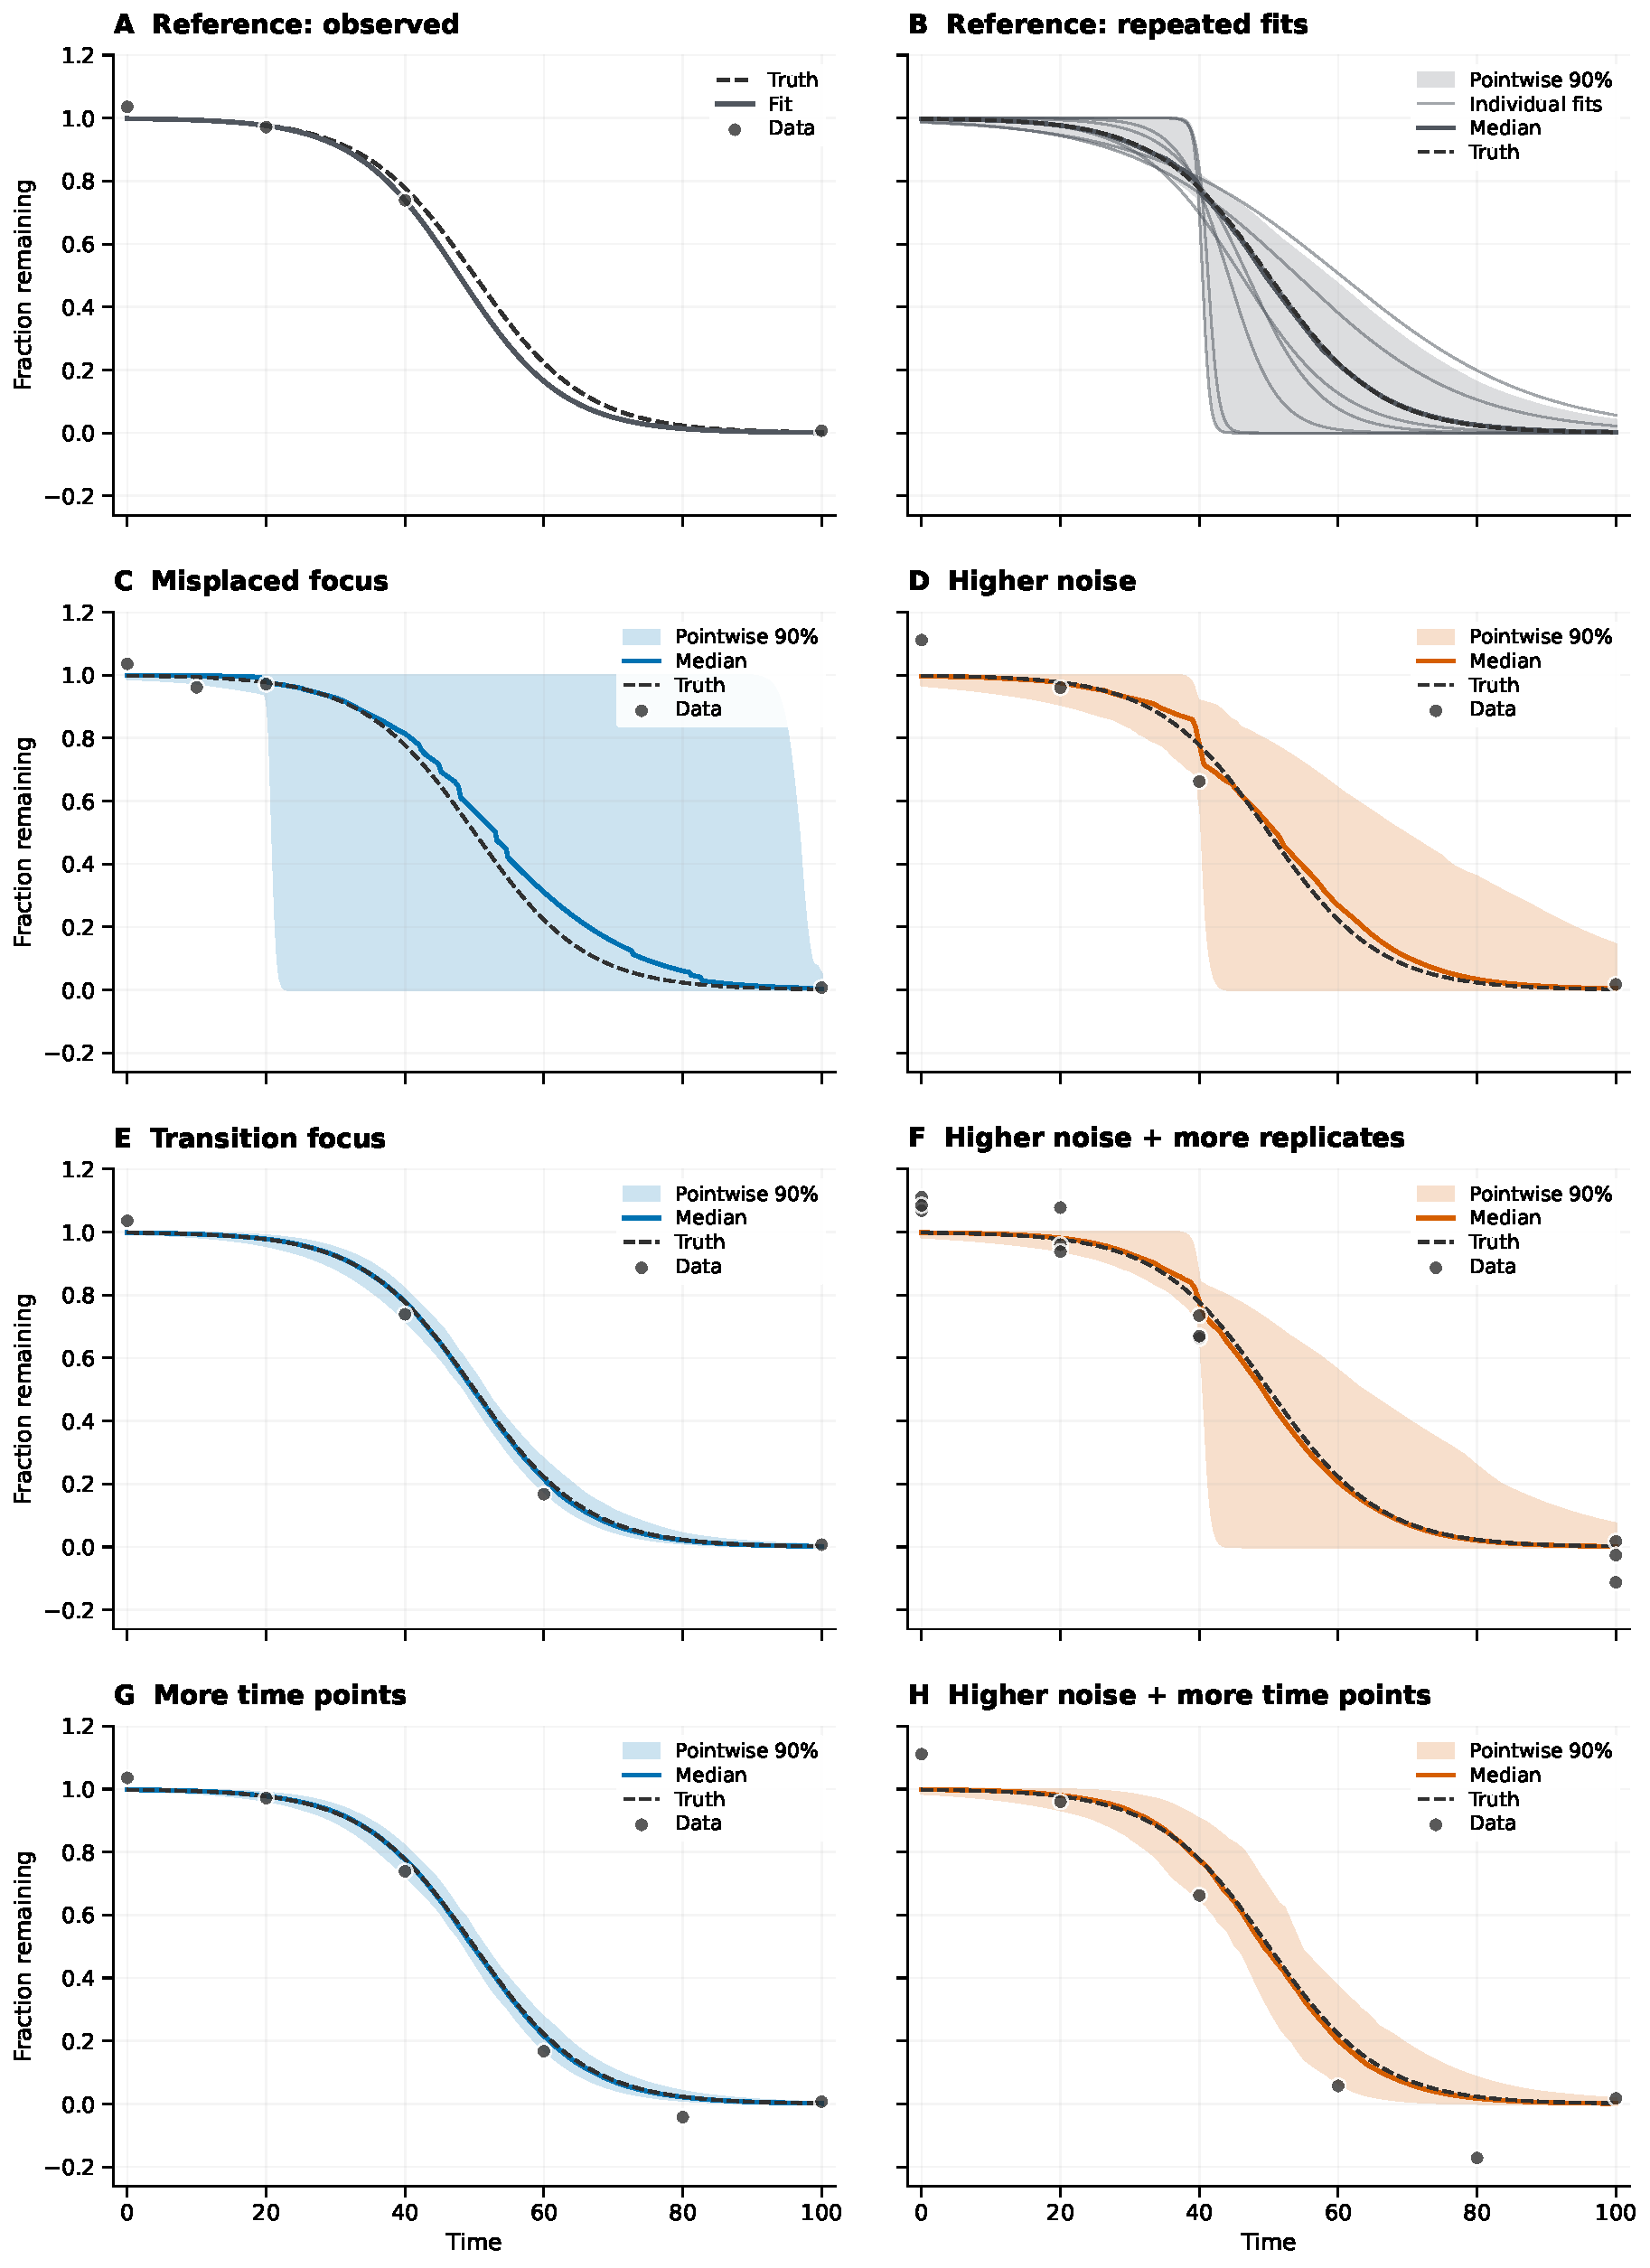
\includegraphics[width=\linewidth,height=0.84\textheight,keepaspectratio]
    {tutorial/sampling_design_01.pdf}
  \caption{Recovery of the known logistic decay under different sampling
    conditions. A shows one study and its fitted curve. In B--H, the line and
    shaded area show the pointwise median and middle 90\% of fitted curves across
    100 repeated studies. Points in C--H come from the separate illustrative
    study. B also shows selected individual fits spanning the observed shape
    variation; these are not frequency-weighted examples. The shaded areas
    describe variation between simulated studies, not the app's 95\%
    parameter-uncertainty bands, observation prediction intervals, or
    cross-validation variability from one dataset.}
  \label{fig:sampling-design-curves}
\end{figure}

\subsection{Recognizing weak support in the app}

Figure~\ref{fig:sampling-design-uncertainty} summarizes the approximate 95\%
confidence-interval half-width for $t_{50}$, the same type of interval shown
in the app's parameter tables. It describes uncertainty in this one fitted
parameter, rather than the shaded curve intervals shown in the app. The reference
and misplaced-focus schedules often give wide
or unavailable intervals. Transition-focused and denser sampling give much
narrower intervals; denser sampling generally narrows them further. Under higher
noise, adding times gives more consistently narrow intervals than adding
replicates at the reference times. The latter still produces some extremely wide
intervals, even though a numerical interval can be calculated.

These are local approximations based on fitted-parameter covariance, and can be
unreliable with sparse data. The boxplots summarize only available intervals;
unavailable intervals in the reference, misplaced-focus, and higher-noise cases
can also signal weak support. A narrow interval alone does not establish that the
curve form is appropriate.

\begin{figure}[htbp]
  \centering
  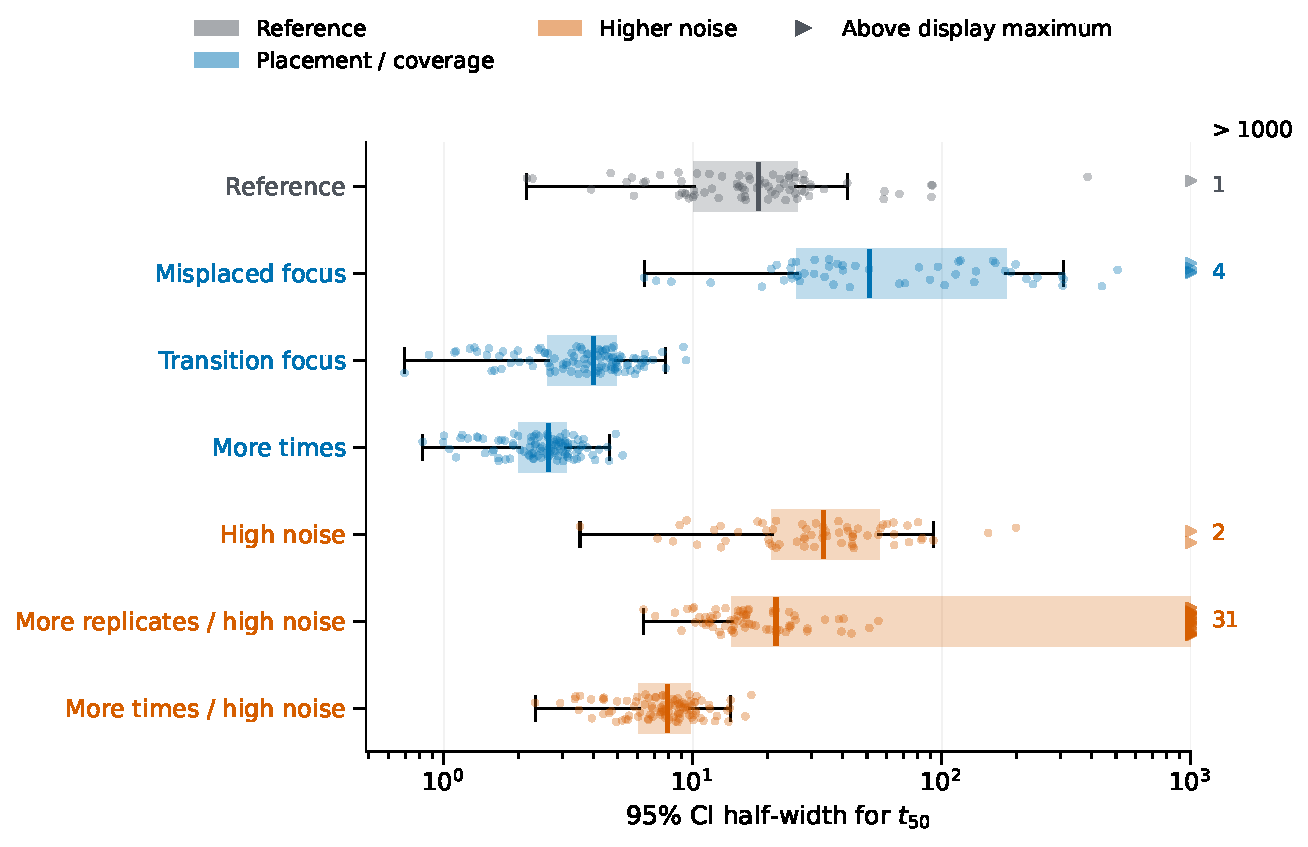
\includegraphics[width=\linewidth]
    {tutorial/sampling_design_02.pdf}
  \caption{Uncertainty in the fitted transition time. Each point represents an
    available local 95\% confidence-interval half-width for $t_{50}$ from one
    repeated study; boxes summarize their distribution. Smaller values indicate
    more precise estimates under the fitted model. The horizontal axis is
    logarithmic. Right-edge triangles and counts mark values above the display
    limit; unavailable intervals are excluded.}
  \label{fig:sampling-design-uncertainty}
\end{figure}

For an actual dataset, inspect where observations fall relative to the fitted
transition, the uncertainty in parameters describing its timing and width, and
how the curve changes when observations or time points are omitted during
cross-validation. Large parameter uncertainty or strong sensitivity to omissions
can motivate additional sampling. Cross-validation cannot supply observations
within an unsampled gap, and its variability is distinct from the repeated-study
bands shown here.

The favorable transition-focused schedule uses knowledge of where the synthetic
transition occurs. In practice, prior information, pilot observations, or broader
initial coverage can help locate important changes. Comparing candidate schedules
across several plausible transition times and curve shapes would provide a
stronger basis for study planning. This example illustrates that reasoning for
one known curve and error model; it does not identify a universally best schedule.
The same sampling principles apply to other model forms, although useful sampling
times and the size of the improvement will depend on the curve and noise.

%\SamplingTutorialEnd
